% ============================================================================
% Chapitre 3 : R\'egularisation et Techniques de G\'en\'eralisation
% ============================================================================
\chapter{R\'egularisation et Techniques de G\'en\'eralisation}
\label{ch:regularisation}

\noindent\textit{Ce chapitre pr\'esente les techniques fondamentales permettant d'am\'eliorer
la capacit\'e de g\'en\'eralisation des r\'eseaux de neurones profonds. Nous
d\'erivons math\'ematiquement les m\'ethodes de r\'egularisation classiques
(L1, L2, Dropout, Batch Normalization) et explorons les approches modernes
utilis\'ees dans les architectures \'etat de l'art.}\medskip

% ----------------------------------------------------------------------------
\section{Surapprentissage et sous-apprentissage}
\label{sec:overfitting-underfitting}
\index{surapprentissage}\index{sous-apprentissage}

\subsection{D\'ecomposition biais-variance}
\index{biais-variance}

Consid\'erons un mod\`ele $\hat{f}$ entra\^in\'e sur un ensemble
$\mathcal{D} = \{(x_i, y_i)\}_{i=1}^N$ o\`u $y = f(x) + \epsilon$ avec
$\epsilon \sim \mathcal{N}(0, \sigma^2)$.

\begin{mathbox}[title=\textbf{D\'ecomposition biais-variance}]
L'erreur quadratique moyenne en un point $x$ se d\'ecompose comme :
\begin{align}
\E\bigl[(y - \hat{f}(x))^2\bigr]
&= \E\bigl[(f(x) + \epsilon - \hat{f}(x))^2\bigr] \nonumber \\
&= \bigl(f(x) - \E[\hat{f}(x)]\bigr)^2
   + \E\bigl[(\hat{f}(x) - \E[\hat{f}(x)])^2\bigr]
   + \sigma^2 \nonumber \\
&= \underbrace{\text{Biais}^2(\hat{f}(x))}_{\text{erreur syst\'ematique}}
   + \underbrace{\Var(\hat{f}(x))}_{\text{sensibilit\'e aux donn\'ees}}
   + \underbrace{\sigma^2}_{\text{bruit irr\'eductible}}
\label{eq:bias-variance}
\end{align}
\end{mathbox}

\begin{definition}[Surapprentissage (Overfitting)]
Un mod\`ele est en \textbf{surapprentissage} lorsque l'erreur d'entra\^inement
est significativement inf\'erieure \`a l'erreur de test :
$\mathcal{L}_{\text{train}} \ll \mathcal{L}_{\text{test}}$. Cela correspond
\`a une variance \'elev\'ee dans la d\'ecomposition biais-variance.
\end{definition}

\begin{definition}[Sous-apprentissage (Underfitting)]
Un mod\`ele est en \textbf{sous-apprentissage} lorsque l'erreur
d'entra\^inement est elle-m\^eme \'elev\'ee :
$\mathcal{L}_{\text{train}} \approx \mathcal{L}_{\text{test}} \gg \mathcal{L}^*$.
Cela correspond \`a un biais \'elev\'e.
\end{definition}

\begin{center}
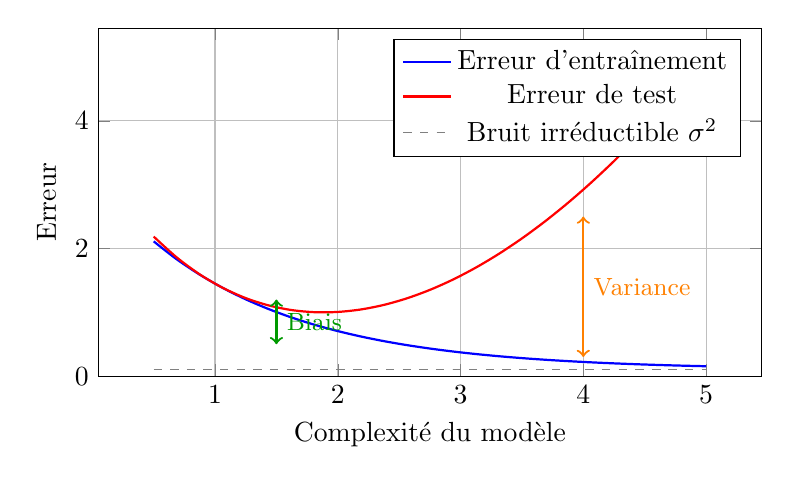
\begin{tikzpicture}
  \begin{axis}[
    width=10cm, height=6cm,
    xlabel={Complexit\'e du mod\`ele},
    ylabel={Erreur},
    legend pos=north east,
    grid=major,
    ymin=0,
    ]
    \addplot[blue, thick, smooth, domain=0.5:5] {3*exp(-0.8*x) + 0.1};
    \addlegendentry{Erreur d'entra\^inement}
    \addplot[red, thick, smooth, domain=0.5:5] {3*exp(-0.8*x) + 0.3*(x-1)^2 + 0.1};
    \addlegendentry{Erreur de test}
    \addplot[dashed, gray, domain=0.5:5] {0.1};
    \addlegendentry{Bruit irr\'eductible $\sigma^2$}
    \draw[<->, thick, green!60!black] (axis cs:1.5,0.5) -- (axis cs:1.5,1.2)
      node[midway, right, font=\small] {Biais};
    \draw[<->, thick, orange] (axis cs:4,0.3) -- (axis cs:4,2.5)
      node[midway, right, font=\small] {Variance};
  \end{axis}
\end{tikzpicture}
\end{center}

% ----------------------------------------------------------------------------
\section{R\'egularisation L2 (Ridge)}
\label{sec:l2-reg}
\index{r\'egularisation!L2}\index{Ridge}

\subsection{Formulation}

La r\'egularisation L2 ajoute une p\'enalit\'e quadratique sur les poids :
\begin{formules}[title=\textbf{Fonction de co\^ut r\'egularis\'ee L2}]
\begin{equation}
\tilde{\mathcal{L}}(\theta) = \mathcal{L}(\theta) + \frac{\lambda}{2} \|\theta\|_2^2
= \mathcal{L}(\theta) + \frac{\lambda}{2} \sum_{i} \theta_i^2
\label{eq:l2-cost}
\end{equation}
\end{formules}

\subsection{D\'erivation du gradient}

Le gradient de la fonction r\'egularis\'ee est :
\begin{align}
\nabla_\theta \tilde{\mathcal{L}}(\theta)
&= \nabla_\theta \mathcal{L}(\theta) + \lambda \theta
\end{align}

La r\`egle de mise \`a jour avec descente de gradient devient :
\begin{align}
\theta_{t+1} &= \theta_t - \eta \nabla_\theta \tilde{\mathcal{L}}(\theta_t) \nonumber \\
&= \theta_t - \eta \nabla_\theta \mathcal{L}(\theta_t) - \eta \lambda \theta_t \nonumber \\
&= (1 - \eta\lambda)\theta_t - \eta \nabla_\theta \mathcal{L}(\theta_t)
\label{eq:l2-update}
\end{align}

Le facteur $(1 - \eta\lambda)$ r\'eduit les poids \`a chaque it\'eration,
d'o\`u le nom <<~weight decay~>>\index{weight decay}.

\subsection{Interpr\'etation g\'eom\'etrique}

\begin{center}
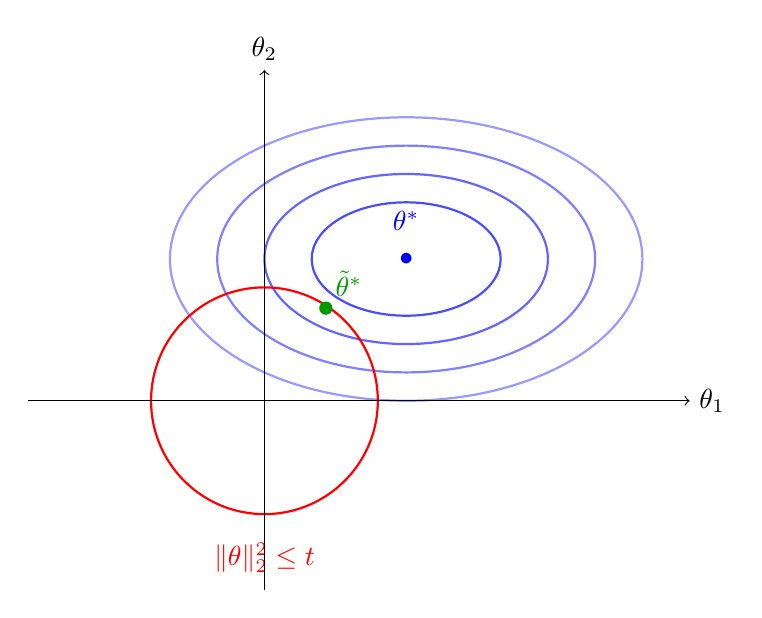
\begin{tikzpicture}[scale=1.2]
  % Contours de la loss
  \draw[blue!40, thick] (1.5, 1.5) ellipse (2.5 and 1.5);
  \draw[blue!50, thick] (1.5, 1.5) ellipse (2.0 and 1.2);
  \draw[blue!60, thick] (1.5, 1.5) ellipse (1.5 and 0.9);
  \draw[blue!70, thick] (1.5, 1.5) ellipse (1.0 and 0.6);
  \node[blue] at (1.5, 1.5) {$\bullet$};
  \node[blue, above] at (1.5, 1.7) {$\theta^*$};

  % Contrainte L2
  \draw[red, thick] (0, 0) circle (1.2);
  \node[red, below] at (0, -1.4) {$\|\theta\|_2^2 \leq t$};

  % Solution r\'egularis\'ee
  \fill[green!60!black] (0.65, 0.98) circle (2pt);
  \node[green!60!black, above right] at (0.65, 1.0) {$\tilde{\theta}^*$};

  % Axes
  \draw[->] (-2.5, 0) -- (4.5, 0) node[right] {$\theta_1$};
  \draw[->] (0, -2) -- (0, 3.5) node[above] {$\theta_2$};
\end{tikzpicture}
\end{center}

\begin{intuition}[title=\textbf{Effet g\'eom\'etrique de L2}]
La r\'egularisation L2 contraint les poids \`a rester dans une boule
euclidienne. La solution r\'egularis\'ee $\tilde{\theta}^*$ se trouve \`a
l'intersection des courbes de niveau de $\mathcal{L}$ et de la sph\`ere
$\|\theta\|_2 = r$.
\end{intuition}

% ----------------------------------------------------------------------------
\section{R\'egularisation L1 (Lasso)}
\label{sec:l1-reg}
\index{r\'egularisation!L1}\index{Lasso}

\begin{formules}[title=\textbf{Fonction de co\^ut r\'egularis\'ee L1}]
\begin{equation}
\tilde{\mathcal{L}}(\theta) = \mathcal{L}(\theta) + \lambda \|\theta\|_1
= \mathcal{L}(\theta) + \lambda \sum_{i} |\theta_i|
\label{eq:l1-cost}
\end{equation}
\end{formules}

Le sous-gradient de la p\'enalit\'e L1 est :
\begin{equation}
\frac{\partial}{\partial \theta_i} \lambda |\theta_i| =
\lambda \cdot \text{sign}(\theta_i) =
\begin{cases}
+\lambda & \text{si } \theta_i > 0 \\
-\lambda & \text{si } \theta_i < 0 \\
[-\lambda, +\lambda] & \text{si } \theta_i = 0
\end{cases}
\end{equation}

\begin{remarque}[Parcimonie de L1]
La r\'egularisation L1 produit des solutions \textbf{parcimonieuses} (sparse) :
certains poids sont exactement z\'ero. G\'eom\'etriquement, la contrainte
$\|\theta\|_1 \leq t$ forme un losange dont les sommets sont align\'es avec
les axes, favorisant les solutions sur les axes de coordonn\'ees.
\end{remarque}

\begin{center}
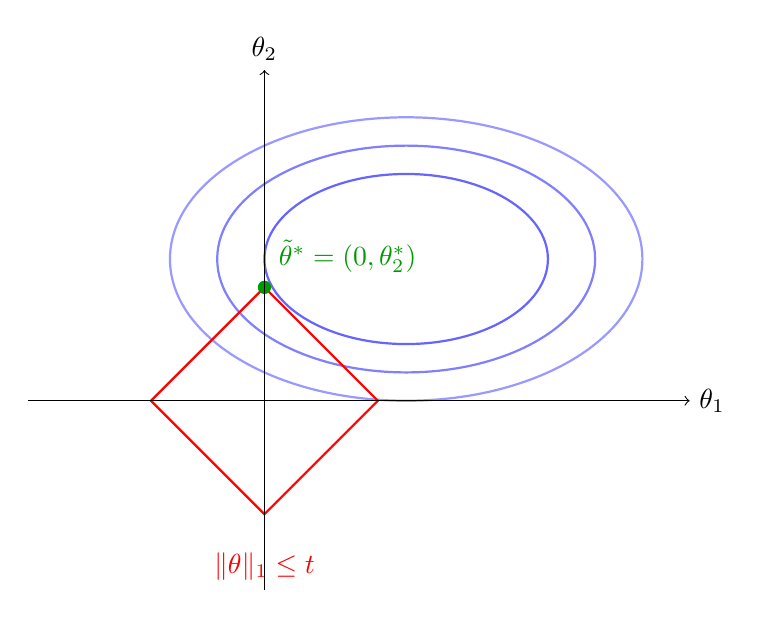
\begin{tikzpicture}[scale=1.2]
  % Contours de la loss
  \draw[blue!40, thick] (1.5, 1.5) ellipse (2.5 and 1.5);
  \draw[blue!50, thick] (1.5, 1.5) ellipse (2.0 and 1.2);
  \draw[blue!60, thick] (1.5, 1.5) ellipse (1.5 and 0.9);

  % Contrainte L1 (losange)
  \draw[red, thick] (1.2, 0) -- (0, 1.2) -- (-1.2, 0) -- (0, -1.2) -- cycle;
  \node[red, below] at (0, -1.5) {$\|\theta\|_1 \leq t$};

  % Solution parcimonieuse
  \fill[green!60!black] (0, 1.2) circle (2pt);
  \node[green!60!black, above right] at (0.05, 1.25) {$\tilde{\theta}^* = (0, \theta_2^*)$};

  % Axes
  \draw[->] (-2.5, 0) -- (4.5, 0) node[right] {$\theta_1$};
  \draw[->] (0, -2) -- (0, 3.5) node[above] {$\theta_2$};
\end{tikzpicture}
\end{center}

% ----------------------------------------------------------------------------
\section{Dropout}
\label{sec:dropout}
\index{Dropout}

\subsection{Masquage de Bernoulli}

Le Dropout \cite{srivastava2014dropout} d\'esactive al\'eatoirement une
fraction $p$ des neurones pendant l'entra\^inement. Pour chaque neurone $j$
de la couche $l$, on \'echantillonne un masque :
\begin{equation}
m_j^{(l)} \sim \text{Bernoulli}(1 - p)
\end{equation}

La sortie masqu\'ee est :
\begin{equation}
\tilde{h}_j^{(l)} = m_j^{(l)} \cdot h_j^{(l)}
\end{equation}

\subsection{Esp\'erance et Dropout invers\'e}
\index{Dropout!invers\'e}

\begin{theoreme}[Esp\'erance du Dropout]
L'esp\'erance de la sortie masqu\'ee est :
\begin{align}
\E[\tilde{h}_j^{(l)}]
&= \E[m_j^{(l)}] \cdot h_j^{(l)} = (1 - p) \cdot h_j^{(l)}
\end{align}
Pour maintenir la m\^eme esp\'erance entre entra\^inement et inf\'erence,
le \textbf{Dropout invers\'e} divise par $(1-p)$ pendant l'entra\^inement :
\begin{equation}
\tilde{h}_j^{(l)} = \frac{m_j^{(l)}}{1 - p} \cdot h_j^{(l)}
\label{eq:inverted-dropout}
\end{equation}
Ainsi $\E[\tilde{h}_j^{(l)}] = h_j^{(l)}$ et aucune modification n'est
n\'ecessaire \`a l'inf\'erence.
\end{theoreme}

\begin{center}
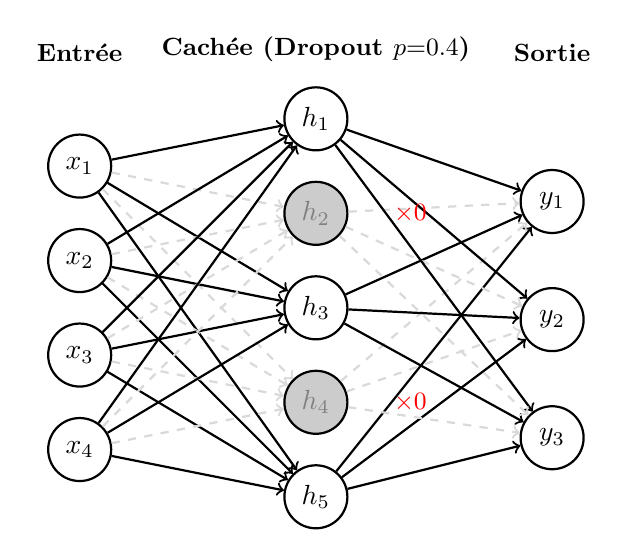
\begin{tikzpicture}[
  neuron/.style={circle, draw, minimum size=8mm, thick},
  dropped/.style={circle, draw, minimum size=8mm, thick, fill=gray!40,
                  text=gray},
  conn/.style={->, thick},
  dropconn/.style={->, thick, gray!30, dashed}
]
  % Couche d'entr\'ee
  \foreach \i in {1,2,3,4} {
    \node[neuron] (i\i) at (0, -\i*1.2) {$x_{\i}$};
  }

  % Couche cach\'ee (avec dropout)
  \node[neuron] (h1) at (3, -0.6) {$h_1$};
  \node[dropped] (h2) at (3, -1.8) {$h_2$};
  \node[neuron] (h3) at (3, -3.0) {$h_3$};
  \node[dropped] (h4) at (3, -4.2) {$h_4$};
  \node[neuron] (h5) at (3, -5.4) {$h_5$};

  % Couche de sortie
  \foreach \i in {1,2,3} {
    \node[neuron] (o\i) at (6, -\i*1.5 - 0.15) {$y_{\i}$};
  }

  % Connexions entr\'ee -> cach\'ee
  \foreach \i in {1,2,3,4} {
    \foreach \j in {1,3,5} {
      \draw[conn] (i\i) -- (h\j);
    }
    \foreach \j in {2,4} {
      \draw[dropconn] (i\i) -- (h\j);
    }
  }

  % Connexions cach\'ee -> sortie
  \foreach \j in {1,2,3} {
    \foreach \h in {1,3,5} {
      \draw[conn] (h\h) -- (o\j);
    }
    \foreach \h in {2,4} {
      \draw[dropconn] (h\h) -- (o\j);
    }
  }

  % Annotations
  \node[above, font=\small\bfseries] at (0, 0) {Entr\'ee};
  \node[above, font=\small\bfseries] at (3, 0) {Cach\'ee (Dropout $p{=}0.4$)};
  \node[above, font=\small\bfseries] at (6, 0) {Sortie};

  \node[red, font=\small] at (4.2, -1.8) {$\times 0$};
  \node[red, font=\small] at (4.2, -4.2) {$\times 0$};
\end{tikzpicture}
\end{center}

% ----------------------------------------------------------------------------
\section{Batch Normalization}
\label{sec:batchnorm}
\index{Batch Normalization}

\subsection{Probl\`eme du d\'ecalage interne des covariables}
\index{d\'ecalage interne des covariables}

L'entra\^inement des r\'eseaux profonds est compliqu\'e par le fait que la
distribution des entr\'ees de chaque couche change \`a mesure que les poids
des couches pr\'ec\'edentes \'evoluent. Ce ph\'enom\`ene, appel\'e
\textit{Internal Covariate Shift} \cite{ioffe2015batch}, ralentit la convergence.

\subsection{Passe avant (Forward)}

Pour un mini-batch $\mathcal{B} = \{x_1, \ldots, x_m\}$ :

\begin{formules}[title=\textbf{Batch Normalization -- Passe avant}]
\begin{align}
\mu_{\mathcal{B}} &= \frac{1}{m} \sum_{i=1}^m x_i
\label{eq:bn-mean} \\
\sigma_{\mathcal{B}}^2 &= \frac{1}{m} \sum_{i=1}^m (x_i - \mu_{\mathcal{B}})^2
\label{eq:bn-var} \\
\hat{x}_i &= \frac{x_i - \mu_{\mathcal{B}}}{\sqrt{\sigma_{\mathcal{B}}^2 + \epsilon}}
\label{eq:bn-norm} \\
y_i &= \gamma \hat{x}_i + \beta \equiv \text{BN}_{\gamma, \beta}(x_i)
\label{eq:bn-output}
\end{align}
o\`u $\gamma$ et $\beta$ sont des param\`etres apprenables, et
$\epsilon > 0$ est un terme de stabilit\'e num\'erique.
\end{formules}

\subsection{Passe arri\`ere (Backward)}

\begin{proposition}[Gradients de la Batch Normalization]
En notant $\frac{\partial \mathcal{L}}{\partial y_i} = \delta_i$, les gradients
de la BatchNorm sont :
\begin{align}
\frac{\partial \mathcal{L}}{\partial \gamma}
  &= \sum_{i=1}^m \delta_i \hat{x}_i \\
\frac{\partial \mathcal{L}}{\partial \beta}
  &= \sum_{i=1}^m \delta_i \\
\frac{\partial \mathcal{L}}{\partial \hat{x}_i}
  &= \delta_i \cdot \gamma \\
\frac{\partial \mathcal{L}}{\partial \sigma_{\mathcal{B}}^2}
  &= \sum_{i=1}^m \frac{\partial \mathcal{L}}{\partial \hat{x}_i}
     \cdot (x_i - \mu_{\mathcal{B}})
     \cdot \left(-\frac{1}{2}\right)(\sigma_{\mathcal{B}}^2 + \epsilon)^{-3/2} \\
\frac{\partial \mathcal{L}}{\partial \mu_{\mathcal{B}}}
  &= \sum_{i=1}^m \frac{\partial \mathcal{L}}{\partial \hat{x}_i}
     \cdot \frac{-1}{\sqrt{\sigma_{\mathcal{B}}^2 + \epsilon}} \\
\frac{\partial \mathcal{L}}{\partial x_i}
  &= \frac{\partial \mathcal{L}}{\partial \hat{x}_i}
     \cdot \frac{1}{\sqrt{\sigma_{\mathcal{B}}^2 + \epsilon}}
   + \frac{\partial \mathcal{L}}{\partial \sigma_{\mathcal{B}}^2}
     \cdot \frac{2(x_i - \mu_{\mathcal{B}})}{m}
   + \frac{\partial \mathcal{L}}{\partial \mu_{\mathcal{B}}} \cdot \frac{1}{m}
\end{align}
\end{proposition}

% ----------------------------------------------------------------------------
\section{Layer Normalization}
\label{sec:layernorm}
\index{Layer Normalization}

Contrairement \`a la Batch Normalization qui normalise sur la dimension du
batch, la Layer Normalization \cite{ba2016layer} normalise sur la dimension
des caract\'eristiques. Pour une entr\'ee $\mathbf{x} \in \R^d$ :

\begin{formules}[title=\textbf{Layer Normalization}]
\begin{align}
\mu &= \frac{1}{d} \sum_{j=1}^d x_j, \qquad
\sigma^2 = \frac{1}{d} \sum_{j=1}^d (x_j - \mu)^2 \\
\text{LN}(\mathbf{x}) &= \gamma \odot \frac{\mathbf{x} - \mu}{\sqrt{\sigma^2 + \epsilon}} + \beta
\end{align}
\end{formules}

\begin{remarque}[BatchNorm vs LayerNorm]
\begin{itemize}
  \item \textbf{BatchNorm} : normalise sur le batch, chaque canal ind\'ependamment.
    Utilis\'e principalement dans les CNN (cf.\ chapitre~\ref{ch:cnn}).
  \item \textbf{LayerNorm} : normalise sur les caract\'eristiques, chaque
    \'echantillon ind\'ependamment. Utilis\'e dans les Transformers
    (cf.\ chapitre~\ref{ch:attention}).
  \item LayerNorm ne d\'epend pas de la taille du batch et fonctionne
    identiquement en entra\^inement et en inf\'erence.
\end{itemize}
\end{remarque}

% ----------------------------------------------------------------------------
\section{Augmentation des donn\'ees}
\label{sec:data-augmentation}
\index{augmentation des donn\'ees}

\subsection{Transformations classiques}

Pour les images : rotations, sym\'etries horizontales, recadrages al\'eatoires,
variations de luminosit\'e, ajout de bruit.

\subsection{Mixup}
\index{Mixup}

\begin{formules}[title=\textbf{Mixup}]
\'Etant donn\'es deux exemples $(x_i, y_i)$ et $(x_j, y_j)$, Mixup
\cite{zhang2018mixup} cr\'ee un nouvel exemple :
\begin{align}
\tilde{x} &= \lambda x_i + (1 - \lambda) x_j \\
\tilde{y} &= \lambda y_i + (1 - \lambda) y_j
\end{align}
o\`u $\lambda \sim \text{Beta}(\alpha, \alpha)$ avec $\alpha > 0$.
\end{formules}

\subsection{CutMix}
\index{CutMix}

\begin{formules}[title=\textbf{CutMix}]
CutMix \cite{yun2019cutmix} remplace une r\'egion rectangulaire de $x_i$ par
la r\'egion correspondante de $x_j$ :
\begin{align}
\tilde{x} &= \mathbf{M} \odot x_i + (1 - \mathbf{M}) \odot x_j \\
\tilde{y} &= \lambda y_i + (1 - \lambda) y_j
\end{align}
o\`u $\mathbf{M} \in \{0, 1\}^{H \times W}$ est un masque binaire et
$\lambda = 1 - \frac{r_w \cdot r_h}{W \cdot H}$ repr\'esente la proportion
de l'image originale.
\end{formules}

% ----------------------------------------------------------------------------
\section{Arr\^et pr\'ecoce (Early Stopping)}
\label{sec:early-stopping}
\index{arr\^et pr\'ecoce}

\begin{definition}[Arr\^et pr\'ecoce]
L'arr\^et pr\'ecoce consiste \`a stopper l'entra\^inement lorsque l'erreur de
validation cesse de diminuer pendant un nombre pr\'ed\'efini d'\'epoques
(<<~patience~>>).
\end{definition}

\begin{theoreme}[\'Equivalence avec la r\'egularisation L2]
Pour un mod\`ele lin\'eaire quadratique avec descente de gradient, l'arr\^et
\`a l'it\'eration $T$ est approximativement \'equivalent \`a une
r\'egularisation L2 avec $\lambda \approx \frac{1}{\eta T}$, o\`u $\eta$ est
le taux d'apprentissage.

\textbf{D\'emonstration} : Soit $\mathcal{L}(\theta) = \frac{1}{2}(\theta - \theta^*)^\top H (\theta - \theta^*)$
avec $H$ la Hessienne. En partant de $\theta_0 = 0$, apr\`es $T$ it\'erations :
\begin{equation}
\theta_T = (I - (I - \eta H)^T) \theta^*
\end{equation}
Pour la r\'egularisation L2, la solution est
$\tilde{\theta} = (H + \lambda I)^{-1} H \theta^*$.
En utilisant la d\'ecomposition spectrale de $H = Q \Lambda Q^\top$, on
montre que les deux solutions co\"incident quand
$1 - (1 - \eta \lambda_i)^T \approx \frac{\lambda_i}{\lambda_i + 1/(\eta T)}$.
\end{theoreme}

% ----------------------------------------------------------------------------
\section{Weight Decay vs L2 dans Adam}
\label{sec:weight-decay-adam}
\index{weight decay!Adam}\index{AdamW}

\begin{attention}[title=\textbf{Diff\'erence cruciale}]
Weight decay et r\'egularisation L2 ne sont \textbf{pas \'equivalents} pour
les optimiseurs adaptatifs comme Adam !
\end{attention}

\subsection{R\'egularisation L2 dans Adam}

Avec L2 dans Adam, le gradient modifi\'e est $g_t = \nabla \mathcal{L}(\theta_t) + \lambda \theta_t$.
Ce gradient est ensuite normalis\'e par les moments d'Adam :
\begin{align}
m_t &= \beta_1 m_{t-1} + (1 - \beta_1)(g_t + \lambda \theta_t) \\
v_t &= \beta_2 v_{t-1} + (1 - \beta_2)(g_t + \lambda \theta_t)^2 \\
\theta_{t+1} &= \theta_t - \eta \frac{\hat{m}_t}{\sqrt{\hat{v}_t} + \epsilon}
\end{align}

Le terme de r\'egularisation $\lambda \theta_t$ est \textbf{att\'enu\'e} par
la normalisation adaptative $\frac{1}{\sqrt{\hat{v}_t} + \epsilon}$.

\subsection{AdamW : Weight Decay d\'ecoupl\'e}

AdamW \cite{loshchilov2019decoupled} applique le weight decay directement :
\begin{formules}[title=\textbf{AdamW}]
\begin{align}
m_t &= \beta_1 m_{t-1} + (1 - \beta_1) g_t \\
v_t &= \beta_2 v_{t-1} + (1 - \beta_2) g_t^2 \\
\theta_{t+1} &= (1 - \eta\lambda)\theta_t
               - \eta \frac{\hat{m}_t}{\sqrt{\hat{v}_t} + \epsilon}
\end{align}
\end{formules}

\begin{bonnepratique}[title=\textbf{Utiliser AdamW}]
En pratique, \textbf{AdamW} (weight decay d\'ecoupl\'e) doit \^etre
pr\'ef\'er\'e \`a Adam avec r\'egularisation L2. AdamW est l'optimiseur
standard pour les Transformers modernes.
\end{bonnepratique}

% ----------------------------------------------------------------------------
\section{Impl\'ementation PyTorch}
\label{sec:reg-pytorch}

\begin{codeblock}[title=\textbf{Boucle d'entra\^inement r\'egularis\'ee compl\`ete}]
\begin{minted}{python}
import torch
import torch.nn as nn
import torch.optim as optim
from torch.utils.data import DataLoader
from torchvision import datasets, transforms

# --- Mod`ele avec Dropout et BatchNorm ---
class RegularizedNet(nn.Module):
    def __init__(self, input_dim=784, hidden_dim=256,
                 num_classes=10, dropout_rate=0.5):
        super().__init__()
        self.layers = nn.Sequential(
            nn.Linear(input_dim, hidden_dim),
            nn.BatchNorm1d(hidden_dim),
            nn.ReLU(),
            nn.Dropout(p=dropout_rate),
            nn.Linear(hidden_dim, hidden_dim),
            nn.BatchNorm1d(hidden_dim),
            nn.ReLU(),
            nn.Dropout(p=dropout_rate),
            nn.Linear(hidden_dim, num_classes)
        )

    def forward(self, x):
        return self.layers(x.view(x.size(0), -1))

# --- Configuration ---
device = torch.device('cuda' if torch.cuda.is_available() else 'cpu')
model = RegularizedNet(dropout_rate=0.3).to(device)

# AdamW avec weight decay d'ecoupl'e
optimizer = optim.AdamW(model.parameters(), lr=1e-3,
                        weight_decay=1e-4)
criterion = nn.CrossEntropyLoss(label_smoothing=0.1)
scheduler = optim.lr_scheduler.CosineAnnealingLR(optimizer, T_max=50)

# --- Data augmentation ---
transform_train = transforms.Compose([
    transforms.RandomRotation(10),
    transforms.RandomAffine(0, translate=(0.1, 0.1)),
    transforms.ToTensor(),
    transforms.Normalize((0.1307,), (0.3081,))
])

train_dataset = datasets.MNIST(root='./data', train=True,
                               transform=transform_train, download=True)
train_loader = DataLoader(train_dataset, batch_size=128, shuffle=True)
val_loader = DataLoader(
    datasets.MNIST(root='./data', train=False,
                   transform=transforms.Compose([
                       transforms.ToTensor(),
                       transforms.Normalize((0.1307,), (0.3081,))
                   ])),
    batch_size=256, shuffle=False
)

# --- Early Stopping ---
class EarlyStopping:
    def __init__(self, patience=10, min_delta=1e-4):
        self.patience = patience
        self.min_delta = min_delta
        self.counter = 0
        self.best_loss = float('inf')
        self.should_stop = False

    def __call__(self, val_loss):
        if val_loss < self.best_loss - self.min_delta:
            self.best_loss = val_loss
            self.counter = 0
        else:
            self.counter += 1
            if self.counter >= self.patience:
                self.should_stop = True

early_stopping = EarlyStopping(patience=10)

# --- Boucle d'entra^inement ---
for epoch in range(50):
    model.train()
    train_loss = 0.0
    for inputs, targets in train_loader:
        inputs, targets = inputs.to(device), targets.to(device)
        optimizer.zero_grad()
        outputs = model(inputs)
        loss = criterion(outputs, targets)
        loss.backward()
        torch.nn.utils.clip_grad_norm_(model.parameters(), max_norm=1.0)
        optimizer.step()
        train_loss += loss.item()

    # Validation
    model.eval()
    val_loss = 0.0
    correct = 0
    with torch.no_grad():
        for inputs, targets in val_loader:
            inputs, targets = inputs.to(device), targets.to(device)
            outputs = model(inputs)
            val_loss += criterion(outputs, targets).item()
            correct += (outputs.argmax(1) == targets).sum().item()

    val_loss /= len(val_loader)
    accuracy = correct / len(val_loader.dataset)
    scheduler.step()

    print(f"Epoch {epoch+1}: train_loss={train_loss/len(train_loader):.4f}, "
          f"val_loss={val_loss:.4f}, accuracy={accuracy:.4f}")

    early_stopping(val_loss)
    if early_stopping.should_stop:
        print("Arr^et pr'ecoce d'eclench'e.")
        break
\end{minted}
\end{codeblock}

% ----------------------------------------------------------------------------
\section{\'Etude d'ablation}
\label{sec:reg-ablation}

\begin{codeblock}[title=\textbf{\'Etude d'ablation : taux de Dropout et Weight Decay}]
\begin{minted}{python}
import itertools
import pandas as pd

results = []
dropout_rates = [0.0, 0.1, 0.3, 0.5, 0.7]
weight_decays = [0.0, 1e-5, 1e-4, 1e-3, 1e-2]

for dr, wd in itertools.product(dropout_rates, weight_decays):
    model = RegularizedNet(dropout_rate=dr).to(device)
    optimizer = optim.AdamW(model.parameters(), lr=1e-3,
                            weight_decay=wd)
    # Entra^iner pendant 20 'epoques (simplifi'e)
    for epoch in range(20):
        model.train()
        for inputs, targets in train_loader:
            inputs, targets = inputs.to(device), targets.to(device)
            optimizer.zero_grad()
            loss = criterion(model(inputs), targets)
            loss.backward()
            optimizer.step()

    # 'Evaluer
    model.eval()
    correct = 0
    with torch.no_grad():
        for inputs, targets in val_loader:
            inputs, targets = inputs.to(device), targets.to(device)
            correct += (model(inputs).argmax(1) == targets).sum().item()
    acc = correct / len(val_loader.dataset)
    results.append({'dropout': dr, 'weight_decay': wd, 'accuracy': acc})

df = pd.DataFrame(results)
pivot = df.pivot(index='dropout', columns='weight_decay', values='accuracy')
print(pivot.to_string(float_format='{:.4f}'.format))
\end{minted}
\end{codeblock}

\begin{codeoutput}
\begin{verbatim}
weight_decay    0.0     1e-05   0.0001  0.001   0.01
dropout
0.0           0.9812  0.9821  0.9835  0.9801  0.9754
0.1           0.9838  0.9842  0.9851  0.9828  0.9773
0.3           0.9845  0.9849  0.9856  0.9839  0.9790
0.5           0.9831  0.9835  0.9843  0.9821  0.9779
0.7           0.9762  0.9770  0.9778  0.9755  0.9701
\end{verbatim}
\end{codeoutput}

\begin{remarque}[Observations]
\begin{itemize}
  \item Le Dropout \`a $p=0.3$ avec weight decay $\lambda=10^{-4}$ donne les
    meilleurs r\'esultats sur MNIST.
  \item Un Dropout trop \'elev\'e ($p=0.7$) d\'egrade les performances en
    limitant trop la capacit\'e du r\'eseau.
  \item Le weight decay \`a $10^{-2}$ est trop agressif et nuit aux performances
    pour tous les taux de Dropout.
\end{itemize}
\end{remarque}

% ----------------------------------------------------------------------------
\section{Techniques \'etat de l'art}
\label{sec:reg-sota}

\begin{sota}[title=\textbf{Techniques de r\'egularisation modernes}]
\begin{description}
  \item[Stochastic Depth] \cite{huang2016deep} : d\'esactive al\'eatoirement
    des blocs r\'esiduels entiers (voir chapitre~\ref{ch:cnn}). Chaque bloc
    $l$ a une probabilit\'e de survie $p_l = 1 - \frac{l}{L}(1 - p_L)$.
    \index{Stochastic Depth}

  \item[DropPath] : variante de Stochastic Depth appliqu\'ee par chemin
    dans les architectures multi-branches. Utilis\'e dans EfficientNet et
    les Vision Transformers.
    \index{DropPath}

  \item[Label Smoothing] \cite{szegedy2016rethinking} : remplace les cibles
    one-hot par :
    \begin{equation}
      y_k^{\text{LS}} = (1 - \alpha) y_k + \frac{\alpha}{K}
    \end{equation}
    o\`u $K$ est le nombre de classes et $\alpha \in [0, 1]$ le param\`etre
    de lissage (typiquement $\alpha = 0.1$).
    \index{Label Smoothing}

  \item[R-Drop] \cite{wu2021r} : minimise la divergence KL entre deux passes
    forward avec Dropout diff\'erent :
    \begin{equation}
      \mathcal{L}_{\text{R-Drop}} = \mathcal{L}_{\text{CE}}
        + \alpha \cdot \frac{1}{2}\bigl(\KL(p_1 \| p_2) + \KL(p_2 \| p_1)\bigr)
    \end{equation}
    \index{R-Drop}
\end{description}
\end{sota}

% ----------------------------------------------------------------------------
\section{Exercices}
\label{sec:reg-exercices}

\begin{exercice}[D\'ecomposition biais-variance \hfill $\bigstar$]
Soit $f(x) = \sin(\pi x)$ et $\hat{f}$ un polyn\^ome de degr\'e $d$ ajust\'e
sur $N = 10$ points bruit\'es ($\sigma = 0.3$).
\begin{enumerate}
  \item D\'emontrer la d\'ecomposition biais-variance (\'equation~\ref{eq:bias-variance}).
  \item Simuler en Python l'erreur pour $d \in \{1, 3, 5, 9, 15\}$ sur 100
    jeux de donn\'ees. Tracer biais$^2$, variance et erreur totale.
  \item Quel degr\'e offre le meilleur compromis ?
\end{enumerate}
\end{exercice}

\begin{exercice}[R\'egularisation Elastic Net \hfill $\bigstar\bigstar$]
L'Elastic Net combine L1 et L2 :
$\Omega(\theta) = \alpha \|\theta\|_1 + \frac{1-\alpha}{2}\|\theta\|_2^2$.
\begin{enumerate}
  \item D\'eriver la r\`egle de mise \`a jour avec descente de gradient
    proximale pour la partie L1.
  \item Impl\'ementer cette r\'egularisation en PyTorch en modifiant
    manuellement les gradients.
  \item Comparer les solutions avec L1 seul, L2 seul, et Elastic Net sur un
    probl\`eme de r\'egression lin\'eaire avec $p = 100$ variables dont 10
    pertinentes.
\end{enumerate}
\end{exercice}

\begin{exercice}[Dropout comme ensemble de mod\`eles \hfill $\bigstar\bigstar$]
\begin{enumerate}
  \item Montrer qu'un r\'eseau avec Dropout de taux $p$ sur $n$ unit\'es
    impl\'emente implicitement un ensemble de $2^n$ sous-r\'eseaux.
  \item Pour un r\'eseau \`a une couche cach\'ee ($d$ unit\'es) avec Dropout,
    d\'eriver l'approximation de la moyenne g\'eom\'etrique du poids
    $W_{\text{test}} = (1-p) W_{\text{train}}$.
  \item Impl\'ementer le MC-Dropout (Monte Carlo Dropout) pour estimer
    l'incertitude pr\'edictive et comparer avec le Dropout standard sur
    un probl\`eme de r\'egression.
\end{enumerate}
\end{exercice}

\begin{exercice}[Impl\'ementation de BatchNorm \`a partir de z\'ero \hfill $\bigstar\bigstar\bigstar$]
\begin{enumerate}
  \item Impl\'ementer la Batch Normalization compl\`ete (forward et backward)
    sans utiliser \texttt{nn.BatchNorm1d}.
  \item V\'erifier la correction du backward avec \texttt{torch.autograd.gradcheck}.
  \item Comparer la vitesse de convergence avec et sans BatchNorm sur CIFAR-10.
  \item \'Etudier l'effet de la taille du batch sur la stabilit\'e de BatchNorm
    (batch sizes : 4, 16, 64, 256).
\end{enumerate}
\end{exercice}

\begin{exercice}[AdamW vs Adam + L2 \hfill $\bigstar\bigstar\bigstar$]
\begin{enumerate}
  \item D\'emontrer formellement que pour SGD, weight decay et L2 sont
    \'equivalents avec $\lambda_{\text{wd}} = \frac{\lambda_{L2}}{\eta}$.
  \item Montrer que cette \'equivalence ne tient plus pour Adam en exhibant
    un contre-exemple analytique (mod\`ele \`a 2 param\`etres avec des
    magnitudes de gradient tr\`es diff\'erentes).
  \item Entra\^iner un mod\`ele Transformer (petit) avec Adam+L2 et AdamW,
    en variant le coefficient de r\'egularisation. Tracer les courbes de
    g\'en\'eralisation et comparer.
\end{enumerate}
\end{exercice}
